\section{Lattice Cryptography}


\subsection{The need for Quantum Resistant Cryptography}
In previous sections, we have seen constructions for asymmetric cryptography based on hardness assumptions like the RSA factoring assumption and the discrete logarithm problem. While these problems are assumed to the hard for classical machines, fast quantum algorithms are known. At a high level, quantum computers use phenomenon from quantum mechanism such as superimposition and entanglement to perform computations. 
In 1994, Peter Shor gave a quantum algorithm \cite{Shor1994} to factor composite number $N$ that runs in $\mathcal{O}\left( (\log N)^2(\log \log N) (\log \log \log N)\right)$. Variations of this algorithm can also be used to compute discrete logarithms even for elliptic curves. Contrast this with the fastest classical algorithm which runs in $O(e^{1.9 (\log N)^{1/3} (\log \log N)^{2/3}})$. Shor's quantum algorithm achieves an exponential speedup over classical algorithms allowing quantum computers to break all previously discussed asymmetric schemes in polynomial time. 

Although quantum computers are expensive and not readily available today, many consider their advent inevitable spawning new research into so called ``quantum-resistant'' or ``post-quantum'' cryptography. In this section, we introduce a new asymmetric encryption scheme based on lattice problems that are assumed to be hard even for quantum computers.  

\subsection{Introduction to Lattices}
This section provides a brief introduction to the theory of lattices in the context of cryptography.
\begin{definition}
(Lattice)
Suppose that $\varvect{B} = \{\varvect{b_1},...,\varvect{b_m}\}$ is a set of $m$ linearly independent vectors in $\reals^n$. The lattice generated by $\varvect{B}$, denoted by $\lattice(\varvect{B})$ is defined as
\[
\lattice(\varvect{B}) = \left\{ \varvect{v} = \sum_{i=1}^m x_i \cdot \varvect{b}_i \; : \; x_i \in \Z \right\}
\]
The integer $m$ is called the rank of the lattice. The lattice $\lattice(\varvect{B}) \subseteq \reals^n$ is an additive subgroup of $\reals^n$. Note that every lattice is a finitely generated free-$\Z$-module and is therefore group-isomorphic to $\Z^m$ 
\end{definition}

\noindent For our purpose, henceforth, we only consider full-rank lattices, i.e. lattices with $m = n$

\begin{remark}
The basis of a lattice is not unique. For example, both $ \{ [0,1],[1,0] \}$ and $\{[1,1], [2,1] \}$ are basis for $\Z^2$
\end{remark}

\noindent Let $\norm{v}$ denote the euclidean norm of the vector $\varvect{v}$. The length of the shortest (non-zero) vector in the lattice $\lattice$, denoted by $\lambda_1(\lattice)$ is therefore,
\[\lambda_1(\lattice) = \min_{\varvect{v} \in \lattice \setminus \{0\}} \norm{\varvect{v}}
\]

\noindent A natural question is to compute the shortest vector in a given lattice. This is called the Shortest Vector Problem (\textbf{SVP}). A relaxation of this problem useful for cryptography is parametrized by $\gamma$ and asks to find a vector whose norm is at most $\gamma \cdot \lambda_1$

\begin{problem} 
\textnormal{\textbf{(Approximate Shortest Vector Problem: $\svpy$)}}
Given an arbitrary basis $\varvect{B}$ of a lattice $\lattice = \lattice(\varvect{B})$, find a non-zero vector $\varvect{v} \in \lattice$ such that $\norm{\varvect{v}} \leq \gamma \cdot \lambda_1(\lattice(\varvect{B}))$
\end{problem}


\noindent The following decision problem is also used for constructing cryptosystems based on lattices.

\begin{problem}
\textnormal{\textbf{(Decisional Approximate SVP: $\gapsvpy$)}}
Given an arbitrary basis $\varvect{B}$ of a lattice $\lattice = \lattice(\varvect{B})$, determine whether $\lambda_1(\lattice) \leq 1$ or $\lambda_1(\lattice) > \gamma$. 

\noindent Note that in situations when $\lambda_1$ is between 1 and $\gamma$, the algorithm is allowed to output either answer. 
\end{problem}

\begin{figure}[h]
\captionsetup[subfigure]{labelformat=empty}
\centering
    \begin{subfigure}[h]{0.45\textwidth}
    \centering
        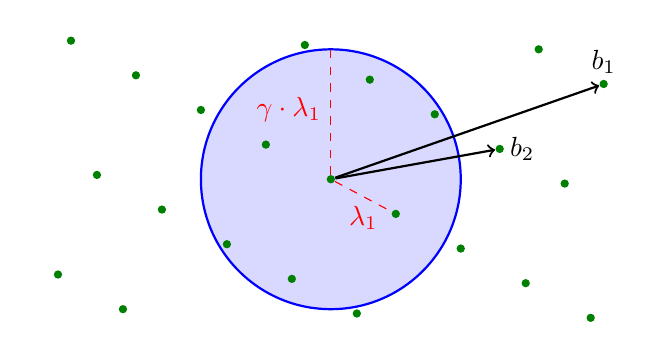
\begin{tikzpicture}[scale=0.55]
            \useasboundingbox (-7,-3.5) rectangle (7,3.5);
            \definecolor{darkgreen}{rgb}{0.0, 0.5, 0.0}
            \def\xdiff{1.5} \def\ydiff{-0.8} \def\rowx{2.4} \def\rowy{1.5}
            \draw [blue,thick,radius=3cm, fill=blue!15] (0, 0) circle;
            \foreach \i in {-2, ..., 2}
                 \foreach \j in {-4, ..., 4} {
                    \def\x{\i * \rowx + \xdiff * \j} \def\y{\i * \rowy + \ydiff * \j}
                    \pgfmathsetmacro{\XALLOW}{abs(\x) < 6.5 ? int(1) : int(0)}
                    \pgfmathsetmacro{\YALLOW}{abs(\y) < 3.5 ? int(1) : int(0)}
                 
                    \ifnum \XALLOW=1
                        \ifnum \YALLOW=1
                            \node[circle,fill=darkgreen,inner sep=0pt,minimum size=3pt] (\i-\j) at (\x,\y) {};
                        \else;\fi
                    \else;\fi
                }
            \draw[dashed,color=red] (0-0)--(0,3.1) node[midway, left] {$\gamma \cdot \lambda_1$};
            \draw[dashed,color=red] (0-0)--(0-1) node[midway,below] {$\lambda_1$};
            \draw[thick,color=black,->] (0-0)--(2-1) node[above] {$\varvect{b}_1$};
            \draw[thick,color=black,->] (0-0)--(1-1) node[right] {$\varvect{b}_2$};
        \end{tikzpicture}
        \caption{$\svpy$}
    \end{subfigure}
    \hfill
    \begin{subfigure}[h]{0.45\textwidth}
        \begin{tikzpicture}[scale=0.55]
            \useasboundingbox (-7,-3.5) rectangle (7,3.5);
            \definecolor{darkgreen}{rgb}{0.0, 0.5, 0.0}
            \def\xdiff{0.25} \def\ydiff{-1.1} \def\rowx{3.5} \def\rowy{-0.5}
            \draw [blue,thick,radius=1.5cm] (0, 0) circle;
            \draw [blue,thick,radius=3cm] (0, 0) circle;
            \foreach \i in {-2, ..., 2}
                 \foreach \j in {-4, ..., 4} {
                    \def\x{\i * \rowx + \xdiff * \j} \def\y{\i * \rowy + \ydiff * \j}
                    \pgfmathsetmacro{\XALLOW}{abs(\x) < 7 ? int(1) : int(0)}
                    \pgfmathsetmacro{\YALLOW}{abs(\y) < 3.5 ? int(1) : int(0)}
                 
                    \ifnum \XALLOW=1
                        \ifnum \YALLOW=1
                            \node[circle,fill=darkgreen,inner sep=0pt,minimum size=3pt] (\i-\j) at (\x,\y) {};
                        \else;\fi
                    \else;\fi
                }
            \draw[dashed,color=red] (0-0)--(0--1) node[midway,left]{$\lambda_1$} ;
            \draw[dashed,color=red] (0-0)--(3.1,0) node[shift={(-0.5,-0.3)}]{ $\gamma$};
            \draw[dashed,color=red] (0-0)--(-1.5,-0.5) node[shift={(0.5,-0.1)}]{$1$};
            \draw[thick,color=black,->] (0-0)--(2-1) node[above] {$\varvect{b}_1$};
            \draw[thick,color=black,->] (0-0)--(1--2) node[above] {$\varvect{b}_2$};
        \end{tikzpicture}
        \caption{$\gapsvpy$}
    \end{subfigure}
    \caption{Lattice Problems}
\end{figure}

\noindent It is known that $\gapsvpy \Rightarrow \svpy$. To build cryptosystems, the strategy is to find constructions whose security reduces first to the $\gapsvpy$ problem rather than directly to $\svpy$. It is easy to see that $\gapsvpy$ and $\svpy$ both get easier as $\gamma$ increases. 
Figure \ref{fig:SVP for Gamma} shows the complexity of the best known algorithms for $\gapsvpy$ for different values of $\gamma$.

\begin{figure}[h]
    \centering
    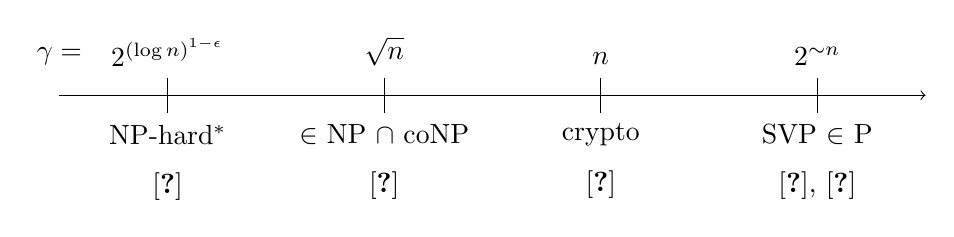
\begin{tikzpicture}[scale=0.55]
    \draw[->] (-10,0) -- (10,0);
    \node[shift={(0,-0.5)},label={[shift={(0,0.5)}]$2^{(\log n)^{1-\epsilon}}$}, label={[shift={(0,-1.2)}]\cite{Ajtai1998}}] (1) at (-7.5,0) {\textrm{NP-hard}$^*$};
    \node[shift={(0,-0.5)},label={[shift={(0,0.5)}]$\sqrt{n}$}, label={[shift={(0,-1.2)}]\cite{Goldreich1998}}] (2) at (-2.5,0) {$\in$ \textrm{NP} $\cap$ \textrm{coNP}};
    \node[shift={(0,-0.5)},label={[shift={(0,0.5)}]$n$}, label={[shift={(0,-1.2)}]\cite{Ajtai1996}}] (3) at (2.5,0) {\textrm{crypto}};
    \node[shift={(0,-0.5)},label={[shift={(0,0.5)}]$2^{\sim n}$}, label={[shift={(0,-1.2)}]\cite{Lenstra1982}, \cite{Schnorr1987}}] (4) at (7.5,0) {\textrm{SVP} $\in$ \textrm{P}};
    
    \node[shift={(0,0.5)}] (0) at (-10,0) {$\gamma = $};

    \foreach \i in {1, ..., 4}{
        \def\x{-12.5 + 5*\i}
        \draw[] (\x,-0.4) --(\x,0.4) {};
    }
    \end{tikzpicture}
    \caption{$\gapsvpy$ hardness for various $\gamma$}
    \label{fig:SVP for Gamma}
\end{figure}


\subsection{Learning with Errors Problems}
At a high level, Learning with Errors (LWE) problems ask questions about an underlying secret given a distribution that hides the secret under some ``noise''. This noise or error distribution, denoted by $\chi$ is usually bounded with high probability. The Discrete Gaussian distribution is often used as the error distribution. Two formulations of LWE, a search variant and a decision variant are given below.

\begin{problem}
\textnormal{\textbf{(Search-Learning with Errors: $\searchlwe$)}} Suppose that $\varvect{s}$, called the secret vector is sampled uniformly at random from $\Z^n_q$. Let $\varvect{A} \getsr \Z^{m \times n}_q$ be a random $m \times n$ matrix and $\varvect{e} \getsr \chi^m$ be a ``noise vector'' containing $m$ samples from $\chi$. Compute the secret vector $\varvect{s}$ given $\left(\varvect{A}, \varvect{A}\varvect{s} + \varvect{e} \right)$
\end{problem}

\begin{problem}
\textnormal{\textbf{(Decision-Learning with Errors: $\decisionlwe$)}}
Given $(\varvect{A}, \varvect{D}_b)$ where $\varvect{D}_1 = \varvect{A}\varvect{s} + \varvect{e}$ and $\varvect{D}_0 \getsr \Z^m_q$, find the bit $b$
\end{problem}

\noindent It is easy to see how the decision version can be solved using the search version assuming $\chi$ is distinguishable from a uniform distribution over $\Z_q$. Intuitively, given a solver $\advA$ for $\searchlwe$, we can construct $\advA'$ that solves $\decisionlwe$ as follows: $\advA'$ feeds its input into $\advA$. Compute $\varvect{e} = \varvect{A}\varvect{s} - \varvect{D}_b$ using the $\varvect{s}$ returned by $\advA$. When $b=0$, $\varvect{e}$ will be a uniformly random vector from $\Z^m_q$ and when $b=1$, $\varvect{e}$ will be from $\chi^m$. Perhaps surprisingly, under some restrictions, the search variant can also be solved using the decision variant. Oded Regev showed in \cite{Regev2005} that the search and decision variants of the LWE problem are equivalent when $q$ is a prime that is polynomial in $n$. This result was extended in \cite{Peikert2009} for any $q$ that is a product of distinct primes that are polynomial in $n$.

\begin{remark}
If $\varvect{e}$ is uniform over $\Z^m_q$, then finding $\varvect{s}$ is impossible. At the other extreme, if the error is 0, then the problem reduces to $m$ equations in $n$ unknowns which can be solved using Gaussian elimination to obtain a unique solution when $m \geq n$
\end{remark}

\subsection{LWE as a lattice problem and Regev's construction}
The connection between LWE and lattices stems from the fact that 
the LWE problem can be viewed as a lattice problem. For certain range of parameters, worst-case hardness of $\gapsvpy$ implies LWE. Regev \cite{Regev2005} built a public key encryption scheme for single bit messages that tightly reduces to the $\decisionlwe$ problem. The details of Regev's construction are given below.

\begin{construction}
(\textbf{Regev's Asymmetric Scheme using LWE})
\begin{figure}[h]
\centering
\hfpagesss{.18}{.18}{.25}{
    \underline{$\kg$}\\[1pt]
    $\sk = s \getsr \Z_q^n$\\
    $\varvect{A} \getsr \Z_q^{m \times n}$\\
    $\varvect{e} \getsr \chi^m$\\
    $\pk \gets \varvect{A} \varvect{s} + \varvect{e}$\\
    Ret $((\pk,\varvect{A}),(\sk, \varvect{A}))$
}
{
    \underline{$\enc((\pk,\varvect{A}), b)$}\\[1pt]
    $\varvect{u} \getsr \bits^m$\\
    $c_1 \gets \varvect{u}^{\textnormal{T}} \varvect{A}$\\
    $c_2 \gets \varvect{u}^{\textnormal{T}} \pk + b \lceil q/2 \rceil$\\
    Ret $(c_1, c_2)$
} 
{
    \underline{$\dec((\sk,\varvect{A}), (c_1,c_2))$}\\[1pt]
    $b' \gets c_2 - c_1 \sk$\\
    \textbf{if} $b'$ is closer to $q/2$ than 0 \textbf{then}\\
    \hspace*{1em} $b \gets 1$\\
    \textbf{else} $b \gets 0$\\
    Ret $b$
}
%\caption{Regev's construction}
%\label{fig:Regev's construction}
\end{figure}
\end{construction}

\noindent Regev's construction is different from previously discussed encryption schemes in that the decryption algorithm may not always be correct. Consider the decrypted value $b'$ 
\begin{align*}
b'  &= c_2 - c_1 \varvect{s}\\
    &= \varvect{u}^{\textnormal{T}} \pk + b \lceil q/2 \rceil - \varvect{u}^{\textnormal{T}} \varvect{A}\varvect{s}\\
    &= \varvect{u}^{\textnormal{T}}\varvect{A}\varvect{s} + \varvect{u}^{\textnormal{T}}\varvect{e} + b \lceil q/2 \rceil - \varvect{u}^{\textnormal{T}} \varvect{A}\varvect{s}\\
    &= \varvect{u}^{\textnormal{T}}\varvect{e} + b \lceil q/2 \rceil
\end{align*}

\noindent For $b'$ to be decrypted correctly to $b$, the error term $\varvect{u}^{\textnormal{T}}\varvect{e}$ must be smaller than $q/4$. This is usually accomplished by choosing a (Gaussian) distribution with small enough values for $\chi$.

\subsubsection{Security of Regev's construction}

To show semantic security for Regev's construction, we sketch a game transition in Figure \ref{fig: Security Regev}.

\begin{figure}[h]
\centering
\hfpagesss{0.2}{0.2}{0.25}{
    \underline{$\G_0$}\\[1pt]
    $(\pk,\varvect{A}),(\sk, \varvect{A}) \getsr \kg$\\
    $b \gets \bits$\\
    $(c_1, c_2) \getsr \enc((\pk, \varvect{A}, b))$\\
    $b' \gets \advA(\pk, \varvect{A}, c_1, c_2)$\\
    Ret $(b = b')$
}
{
    \underline{$\G_1$}\\[1pt]
    $(\pk,\varvect{A}),(\sk, \varvect{A}) \getsr \kg$\\
    $\varvect{Z} \gets \Z_q^m$\\
    $b \gets \bits$\\
    $(c_1, c_2) \getsr \enc((\varvect{Z}, \varvect{A}, b))$\\
    $b' \gets \advA(\varvect{Z}, \varvect{A}, c_1, c_2)$\\
    Ret $(b = b')$
}
{
    \underline{$\G_2$}\\[1pt]
    $(\pk,\varvect{A}),(\sk, \varvect{A}) \getsr \kg$\\
    $\varvect{Z} \gets \Z_q^m$\\
    $b \gets \bits$\\
    $\varvect{r_1} \getsr \Z_q^n$; $r_2 \getsr \Z_q$\\
    $b' \gets \advA(\varvect{Z}, \varvect{A}, \varvect{r_1}, r_2 + b \lceil q/2 \rceil)$\\
    Ret $(b = b')$
}
\caption{Security game for Regev's Construction}
\label{fig: Security Regev}
\end{figure}

\noindent Since only one bit is encrypted by the scheme, Game $\G_0$ is equivalent to the $\INDCPA$ game. Game $\G_1$ is the same as $\G_0$ except that the public key is replaced with a random vector $\varvect{Z}$. Now, we can bound the difference between the probability of winning these games by the advantage of a machine $\advB$ in predicting the bit for the decision LWE game. That is,
\[
    \Pr[\G_0] - \Pr[\G_1] \leq \Adv^{\textnormal{dlwe}}(\advB)
\]
Machine $\advB$, given $(\varvect{A}, \varvect{D}_b)$ from its game, first chooses a bit $\hat{b}$ and computes $(c_1, c_2) \getsr \enc(\varvect{D}_b, \varvect{A}, \hat{b})$. $\advB$ then calls $\advA$ with $(\varvect{D}_b, \varvect{A}, c_1, c_2)$ and returns 1 if $\advA$ wins and 0 otherwise. Now, when $b = 1$, $\advB$ wins its game whenever $\advA$ wins in $\G_0$. When $b = 0$, $\advB$ wins whenever $\advA$ wins in $\G_1$.\\

\noindent Now, we use the leftover hash lemma from to show that $\left( \varvect{Z}, \varvect{A}, (\varvect{u}^{\textnormal{T}}\varvect{A}, \varvect{u}^{\textnormal{T}}\varvect{Z}) \right)$ is statistically indistinguishable from $\left(\varvect{Z}, \varvect{A}, (\varvect{r}_1^{\textnormal{T}}, r_2) \right)$ where $(\varvect{r}_1^{\textnormal{T}}, r_2)$ is sampled uniformly at random from $\Z_q^n \times \Z_q$. This means that $\Pr[\G_2] = \Pr[\G_1]$

\noindent Now, since $r_2$ is uniformly sampled from $\Z_q$, $r_2 + b \lceil q/2 \rceil$ is uniformly distributed in $\Z_q$ as well which mean that the bit $b$ is perfectly hidden. Therefore, the probability of $\advA$ winning in $\G_2$ is at most $\frac{1}{2}$. Therefore,
\[
    \Pr[\G_0] = \Adv^{\textnormal{dlwe}}(\advB) + \frac{1}{2}
\]
and we conclude
\[
    \AdvINDCPA{}{\advA} \leq \Adv^{\textnormal{dlwe}}(\advB)
\]


\subsection{Futher Comments and Future Directions}
There are several reasons why Regev's scheme is not practical yet. The constructions requires an $O(n^2)$ public-key size and $O(n)$ elements of $\Z_q$ in the ciphertext. Furthermore, encryption needs to be done bit by bit. An efficient construction that modified the original construction was proposed in \cite{Lyubashevsky2010}. This construction is based on the Ring-LWE problem, an algebraic variant of LWE over a polynomial ring and allows for encryption of the entire $n$ bit message at once. Table \ref{table:LWE Table} shows the key and ciphertext sizes for the \textsc{NewHope-KEM} implementation of the Ring-LWE scheme.

\begin{table}[h]
    \centering
    \begin{tabular}{|c|c|c|c|}
    \hline
    Parameter Set & $\abs{\pk}$ & $\abs{\sk}$ & $\abs{\textnormal{ciphertext}}$\\
    \hline
    \hline
    \textsc{NewHope512-CPA-KEM} & 928 & 869 & 1088\\
    \hline
    \textsc{NewHope1024-CPA-KEM} & 1824 & 1792 & 2176\\
    \hline
    \scshape{NewHope512-CCA-KEM} & 928 & 1888 & 1120\\
    \hline
    \scshape{NewHope1024-CCA-KEM} & 1824 & 3680 & 2208\\
    \hline
    \end{tabular}
    \caption{}
    \label{table:LWE Table}
\end{table}

\noindent The Ring-LWE based scheme is still not as efficient as standard classical schemes in terms of key and ciphertext size for a given security parameter. Figure \ref{fig:ringlwe comparison} shows a comparison between the \textsc{NewHope} Ring-LWE and classical schemes based on RSA or the discrete logarithm problem in ellicptic curve groups. 
\begin{figure}[h!]
    \centering
    \begin{subfigure}[h]{0.5\textwidth}
            \centering
            \begin{tabular}{|c|c|c|}
            \hline
            Security Level & RSA $\log N$ & ECC DL\\
            \hline
            \hline
            80 & 1024 & 160\\
            \hline
            112 & 2048 & 224\\
            \hline
            128 & 3072 & 256\\
            \hline
            256 & 15360 & 512\\
            \hline
            \end{tabular}
    \end{subfigure}
    ~
    \begin{subfigure}[h]{0.4\textwidth}
            \centering
            \begin{tabular}{|p{20mm}|p{20mm}|p{20mm}|}
            \hline
            Security (QC bits) & \textsc{NewHope} $\abs{\pk}$ & \textsc{NewHope} $\abs{\textnormal{ctxt}}$ \\
            \hline
            \hline
            101 & 7424 & 8704\\
            \hline
            233 & 14592 & 17408\\
            \hline
            \end{tabular}
    \end{subfigure}
    \caption{Comparision between Ring-LWE and RSA/ECC DL}
    \label{fig:ringlwe comparison}
\end{figure}

\newpage